\documentclass{article} % For LaTeX2e
\usepackage{xeCJK}  %必须加xeCJK包
\setCJKmainfont{AR PL UMing CN}  %换成本地字体
\usepackage{bm}
\usepackage{nips14submit_e,times}
%\usepackage{hyperref}
\usepackage{url}
\usepackage{amssymb}
\usepackage{amsthm}
\usepackage[numbers]{natbib}
\usepackage{enumitem}
\usepackage{amsmath}  % required if you use \overset
%\documentstyle[nips14submit_09,times,art10]{article} % For LaTeX 2.09
\usepackage{array}
\newtheorem{proposition}{Proposition}
\newtheorem{lemma}{Lemma}
\newtheorem{corollary}{Corollary}
\newtheorem{theorem}{Theorem}
\newtheorem*{thmnonumber}{Theorem}


% For algorithms
\usepackage{algorithm}
\usepackage{algorithmic}

\usepackage{graphicx}
%\usepackage{wrapfigure}
%\usepackage{savetrees}
% Packages hyperref and algorithmic misbehave sometimes.  We can fix
% this with the following command.
\newcommand{\theHalgorithm}{\arabic{algorithm}}




\title{条件生成式对抗网络}


\author{
Mehdi Mirza \\
D\'epartement d'informatique et de recherche op\'erationnelle\\
Universit\'e de Montr\'eal\\
Montr\'eal, QC H3C 3J7 \\
\texttt{mirzamom@iro.umontreal.ca}
\AND
Simon Osindero \\
Flickr / Yahoo Inc. \\
San Francisco, CA 94103 \\
\texttt{osindero@yahoo-inc.com} \\
翻译:张兴园(初),路转(复),管枫(审)\\
}


\newcommand{\fix}{\marginpar{FIX}}
\newcommand{\new}{\marginpar{NEW}}

\nipsfinalcopy % Uncomment for camera-ready version

\begin{document}


\maketitle

\begin{abstract}
\textbf{生成式对抗网络(GAN)}\cite{Goodfellow-et-al-NIPS2014-small}是一种用来训练生成式模型的新方法。本文中,我们在GAN的基础之上引入条件生成式对抗网络,它的构建并不复杂,只需要在生成模型与判别模型的构建中分别输入条件数据y。实验结果显示此模型能够在类别标签条件下生成MNIST手写体数字。对于多模态模型的训练,本文也给出了一个生成图像标记的初步示例,在这个示例中我们演示了如何生成训练标签之外的描述性标签。
\end{abstract}

\section{Introduction}

%-- Brief overview of adversarial nets, and a recap of the motivation for why they are useful.
生成对抗网络(GAN)是最新引入的一种用来训练生成模型的方法,它可以有效的绕过一些其他方法所很难避免的困难的概率计算。

生成网络中不再需要马尔科夫链,而只需要用回溯法就可以计算优化步骤中所需要的梯度向量。在模型训练中也不再需要统计推断,这种方法使得其所训练的模型可以很容易就囊括各种不同类型的信息。

而且,如文章\cite{Goodfellow-et-al-NIPS2014-small}所述,GAN可以实现目前最好的对数似然估计以及生成样本。

%-- Expand motivation to conditional generative models, and explain why this is useful/interesting.
然而,在非条件生成模型中,无法控制其生成数据的模式。使用附加信息作为模型的条件变量,可以引导生成模型的数据生成。这些条件变量可以来自于类别标签,也可以来自于待修复数据的其他部分\cite{goodfellow2013multi},或者甚至来自于其他模态的数据。

%-- Summary of what we intend to demonstrate in this paper (proof of concept on MNIST and images)
本文中我们展示了如何构建条件生成网络,以及条件生成网络在MNIST 手写数字生成以及 MIR Flickr 25,000 图像\cite{huiskes08}的标注生成上的实验结果.

\section{Related Work}
%-- \subsection{Conditional Generative Models}
%-- TODO Do we need this?
%-- We can probably leave conditional generative models out for now

\subsection{多模态学习实现图像标记(标注)}

尽管近来监督神经网络取得很大成功(尤其是卷积神经网络) \cite{Krizhevsky-2012, szegedy2014going},但是对于使用上述模型来预测极其大量的输出类别仍然是一个挑战。其次,迄今为止的大部分工作集中于学习从输入到输出的一对一映射。然而,许多有趣的问题在概率上是一对多的映射问题。例如,图像标记问题,对于给定的一副图像,可能有不同的标签,同时不同的标注者可能使用不同的(但是同义或相关的)词语来描述同一副图像。

解决第一个问题的一种方式是利用其它模态的额外信息:例如,可以使用自然语言语料库来训练标签的向量表示,并保证向量之间的距离远近可以表示语义上含义的远近。在这样的空间进行预测的一个好处是,即使预测有偏差预测结果也能跟真实情况比较”接近”(比如“table”和“chair”),同时这种方法是我们可以预测那些在训练集中没有出现的标签。工作 \cite{frome2013devise} 表明,即使一个从图像特征空间到词表示空间的简单的线性映射也能改善分类效果。

解决第二个问题的方式就是使用条件概率生成模型,在这种模型中输入的是条件变量,这样以来预测一对多的映射就变成了预测条件分布。

%Adversarial nets
%were recently introduced \cite{Goodfellow-et-al-NIPS2014-small} as a novel and effective way to train stochastic generative models, and have several
%appealing properties such as avoiding inference challenges such as explaining-away or evaluating partition functions. In this paper we explore
%the conditional version of adversarial nets as a tool to learn multi-modal mappings from images to labels, and also exploit the fact that by making
%predictions in a semantic feature space we are able to predict labels that were not seen during training.

\cite{Srivastava+Salakhutdinov-NIPS2012-small}采用了类似的方法来解决上述问题,在MIR Flickr25,000数据集上训练了一个多模态深度玻尔兹曼机。

此外,\cite{kiros2013multimodal} 中提到了如何训练一个有监督的多模态神经语言模型,同时能够生成图像的描述性句子。

\section{条件对抗网络}
\subsection{生成式对抗网络}
生成式对抗网络是一种最近引入用来训练生成式模型的全新方式。它由两个“对抗式”模型组成:生成式模型$G$来获取数据分布,判别式模型$D$用来估计一个样本来自与训练集而不是来自于$G$的概率。$G$和$D$都是非线性映射函数,例如多层感知器。

为了学习数据${\bm{x}}$的生成式分布${p_g}$, 生成器构建一个从先验噪声分布 ${p_z(z)}$ 数据空间的映射函数 ${G(z;\theta_g)}$. 判别器 ${D(x; \theta_d)}$ 则输出单个标量来表示 ${\bm{x}}$ 来自训练数据而不是 ${p_g}$ 的概率.

${G}$ 和 ${D}$ 同时进行训练:我们针对 ${G}$ 调整参数来最小化 ${log(1-D(G(\bm{z}))}$ 同时针对 $D$ 调整参数来最小化 ${logD(X)}$, 如同两个玩家使用如下的价值函数 ${V(G, D)}$ 玩最小最大游戏:


\begin{equation}
\label{eq:minimaxgame-definition}
\min_G \max_D V(D, G) = \mathbb{E}_{\bm{x} \sim p_{\text{data}}(\bm{x})}[\log D(\bm{x})] + \mathbb{E}_{\bm{z} \sim p_z(\bm{z})}[\log (1 - D(G(\bm{z})))].
\end{equation}


\subsection{条件对抗网}

如果生成器和判别器都共同的额外条件变量${\bm{y}}$,生成式对抗网络就可以够扩展成条件模型.${\bm{y}}$可以是任何类型的辅助信息,比如类别标签或者其他模态的数据。我们通过将${\bm{y}}$作为额外输入层导入到判别器和生成器来实现条件模型。


在生成器中,先验输入的噪声 $p_{\bm{z}}(\bm{z})$ 和 ${\bm{y}}$在隐藏层中相结合,这使得对抗网络训练框架在如何构成隐藏层方面具有了很大的灵活性。\footnote{在本文中,我们只考虑条件变量与先验噪音共同作为多层感知器的单一隐藏层的输入的情形。但是条件变量与先验噪音的高层交互作用可以产生更复杂的生成器,而这种交互在传统的生成器中是很难实现的}

在判别器中 ${\bm{x}}$ 和 ${\bm{y}}$ 共同做为判别函数的输入(这里仍然考虑在MLP中进行实现的情形).

此处双玩家最小最大游戏的目标函数如下\ref{eq:minimaxgame-definition-conditioned}:
\begin{equation}
\label{eq:minimaxgame-definition-conditioned}
\min_G \max_D V(D, G) = \mathbb{E}_{\bm{x} \sim p_{\text{data}}(\bm{x})}[\log D(\bm{x} | \bm{y})] + \mathbb{E}_{\bm{z} \sim p_z(\bm{z})}[\log (1 - D(G(\bm{z} | \bm{y})))].
\end{equation}

图 \ref{fig:diagram} 展示了简单的条件对抗网络的结构.

\begin{figure}[h]
\centering
    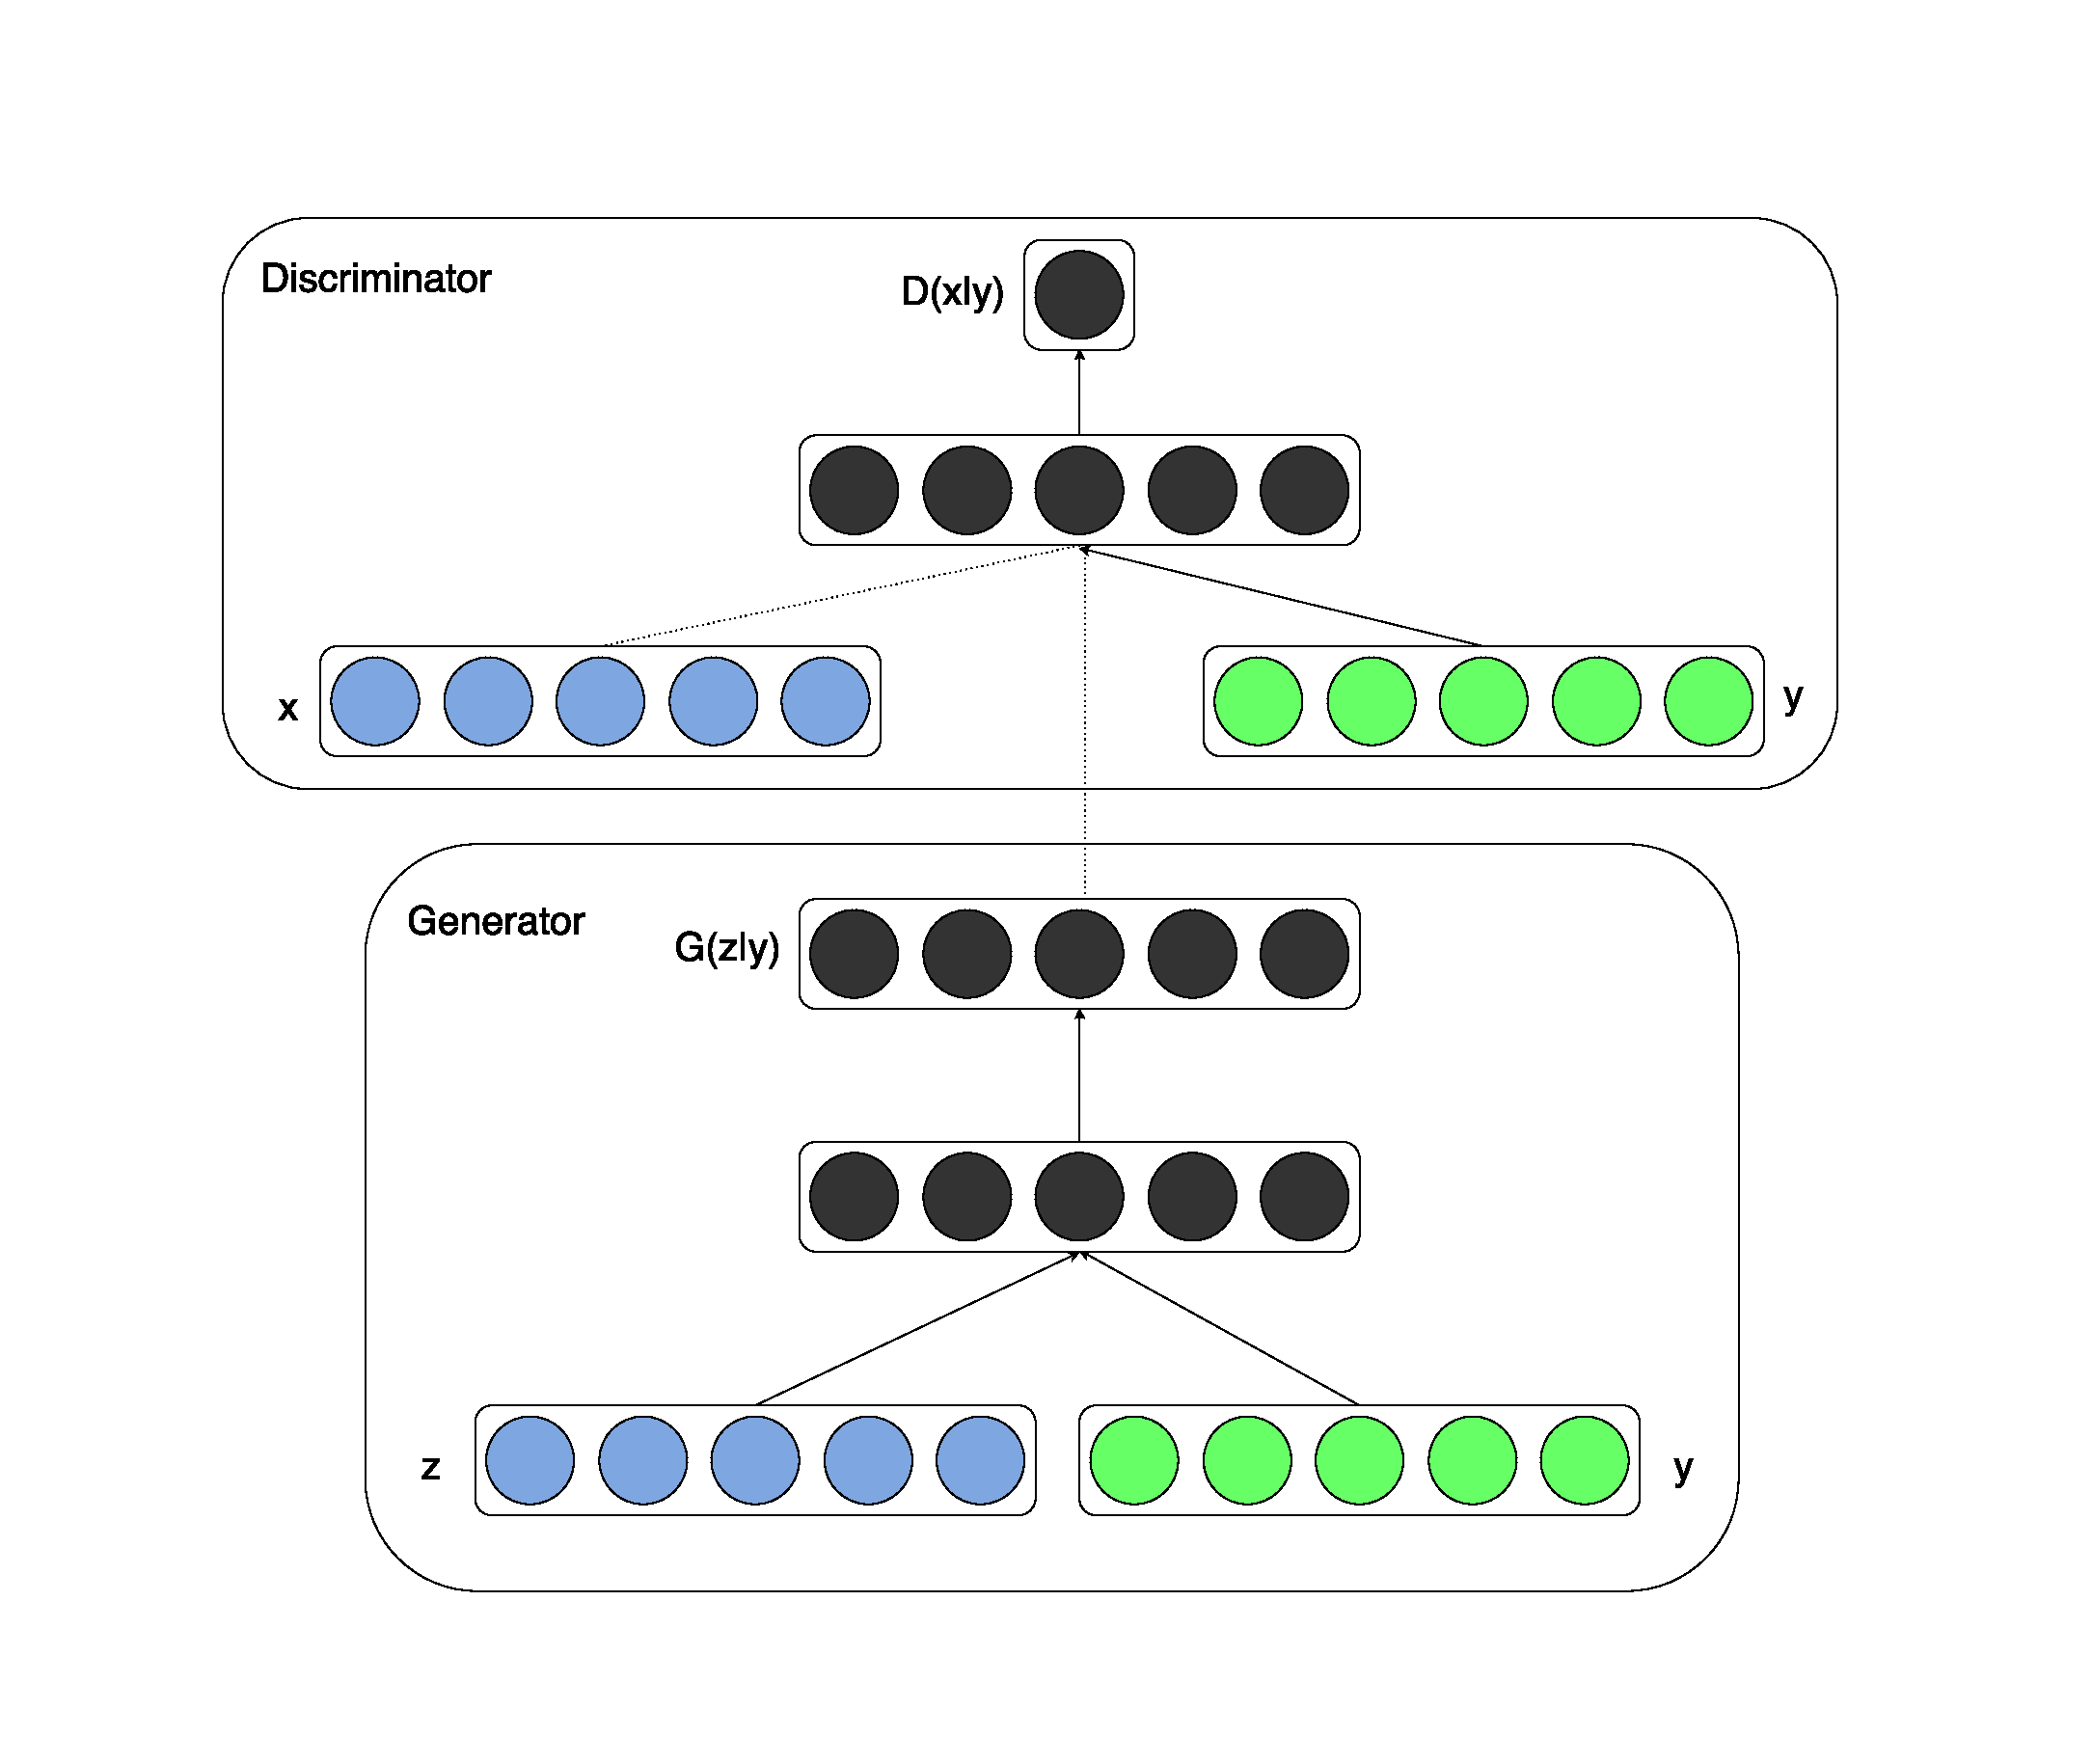
\includegraphics[width=0.9\textwidth]{diagram.pdf}
    \caption{\small 条件对抗网络}
\label{fig:diagram}
\end{figure}


\section{实验结果}
\subsection{单模态}

本文使用标签类别作为条件变量,对编码成one-hot向量的MNIST图像进行条件对抗网络的训练。

在生成式网络部分,我们从单位超立方体上的均匀分布中提取100维的先验噪音${\bm{z}}$。先通过激活函数ReLu(Rectified Linear Unit)\cite{glorot2011deep, Jarrett-ICCV2009-small}把先验噪音${\bm{z}}$和条件变量${\bm{y}}$映射到尺寸分别为200和1000的隐藏层,然后把这两个再映射到1200维的组合ReLu隐藏层,最终在输出层使用sigmoid单元层来生成784维MNIST样本。

判别器把 ${\bm{x}}$ 映射到具有240个单元5块的maxout \cite{Goodfellow_maxout_2013} 层, 把 ${\bm{y}}$ 映射到具有50个单元5块的maxout层. 然后把这两个隐藏层都映射到一个具有240个单元4块的联合隐藏maxout层,最后再把这个层的输出导入sigmoid层. (判别器的具体构造并不关键,只要它具有相当的判别能力就可以,我们实践发现maxout 单元比较适合这个任务)

模型的训练使用随机梯度下降法,其中每个mini-batch的大小为100,学习率初始值为 $0.1$,然后以$1.00004$的下降率指数下降到$.000001$,同时初始动量为 $.5$,最终增长至$0.7$. 为了防止过度拟合,我们在生成器和判别器中的都使用了概率为$0.5$的Dropout层\cite{Hinton-et-al-arxiv2012}.

表格\ref{table:parzen}给出了对于MNIST 数据集的测试数据做的 Gaussian Parzen window 对数-似然估计结果。我们从十个类别中每个类别抽取出来1000个样本进行了Gaussian Parzen window拟合,然后使用Parzen window分布对这个测试集进行对数似然估计。(\cite{Goodfellow-et-al-NIPS2014-small}中有关于如何构造这个估计的更详细讨论)

我们这里使用条件对抗网络得到的结果与一些基于network的构架得出的结果相当,但是却不如一些其他的方法(比如非条件对抗网络).我们此处的结果更多的是作为一个概念验证,但是相信对超参数以及架构的进一步探索可以使得条件生成网络最终达到或者超过非条件生成网络的水平.

图 \ref{fig:mnist} 给出了一些生成的样本. 每一行代表一个条件标签,而每一列代表一个生成样本.

\begin{table}
	\centering
	\begin{tabular}{c|c}
	Model & MNIST  \\
	\hline
	DBN~\citep{Bengio-et-al-ICML2013} & $138 \pm 2$  \\
	Stacked CAE~\citep{Bengio-et-al-ICML2013} & $121 \pm 1.6$ \\
	Deep GSN~\citep{Bengio-et-al-ICML-2014} & $214 \pm 1.1$ \\
	Adversarial nets & $225 \pm 2$ \\
	Conditional adversarial nets & $132 \pm 1.8$
	\end{tabular}
	\caption{\small
	基于Parzen window 对MNIST进行的对数似然估计. 我们使用了和
	\cite{Goodfellow-et-al-NIPS2014-small} 中相同的方法来进行计算.}
	\label{table:parzen}
\end{table}



\begin{figure}[h]
	\centering
	    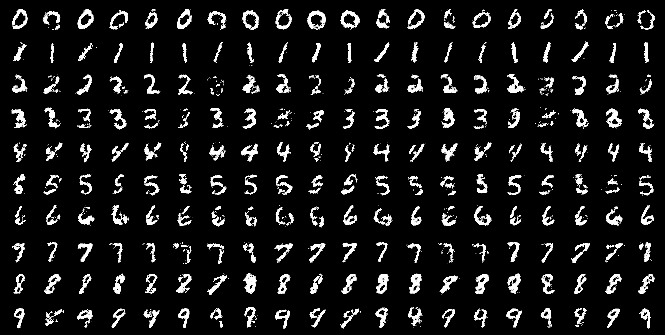
\includegraphics[width=0.9\textwidth]{mnist.png}
	    \caption{\small 生成的 MNIST 手写数据样本,每一行代表一个标签}
	\label{fig:mnist}
\end{figure}



\subsection{多模态}
类似于Flickr 这样的照片网站提供了大量的带标记图像数据以及相关的用户生成的元数据(UGM)特别是用户标签。

用户生成的元数据不同于“规范的”图像标记,因为他们更具有描述性,同时在语义上与人类使用自然语言而不是识别图像中存在的目标实现对图像进行描述更加接近。UGM的另一个方面是同义词非常普遍,同时不同的用户可能使用不同的词汇来描述同一个概念。因此,使用有效的方法来标准化这些标签也就变得非常重要。概念词嵌入方法\cite{mikolov-et-al-iclr2013}就很有效,因为这种方法使得相关的概念最终由相似的向量表示。

我们在本节中以图像特征为条件变量,使用条件生成网络来生成标签向量的条件分布。并以此实现图像的多标签自动标注。

对于图像特征,我们预先在带有21,000个标签的完整ImageNet数据集\cite{RussakovskyFeiFei}上训练一个类似于\cite{Krizhevsky-2012}中的卷积模型。然后使用其具有4096个单元的最后一个全连接层对图像特征进行表示。

对于单词表示,首先从YFCC100M\footnote{Yahoo Flickr Creative Common 100M \url{http://webscope.sandbox.yahoo.com/catalog.php?datatype=i&did=67}.}元数据集中收集了一个混合了用户标签、标题以及描述文本的语料库。经过预处理和文档清理,本文使用大小为200的单词向量进行skip-gram模型拟合。我们过滤掉出现次数少于200次的单词,从而得到一个最终大小为247465的单词表.

我们在训练对抗网络时保持这个卷积模型和语言模型,并把基于这些模型的反向传播算法实验留作今后的工作。

本文的实验对MIR Flickr 25,000数据集\cite{huiskes08},使用如上的卷积模型与语言模型提取了图像与标注特征。我们在实验中过滤掉了没有任何标注的图像,而将附注(annotations)作为额外的标注。实验选取前150,000个例子作为训练集.有多个标注的图像在训练集中重复出现(每一个标注重复一次)。

作为测试,我们对每个图像生成100个样本,并且在每一个样本中使用余弦相似函数选取前20个最接近的词语。然后在100个样本中选取前10个出现最多的词。表格\ref{table:samples}给出了一些用户标注与附注跟生成标注的对比。

表现最好的模型的生成器使用的是如下配置:以100个单位的高斯噪音为先验噪音,然后映射到500维的ReLu层.把4096维的图像特征向量映射到2000维的ReLu隐藏层.这两个ReLu层都映射到一个200维的线性混合表示层,而由这一层来输出词语向量。

判别器包含500维的词语向量隐藏层和1200维的图像特征ReLu隐藏层,这两层映射到一个1000个单元与3块的maxout层,然后最终导入到一个单sigmoid单元,并输出判断.

模型的优化使用的是随机梯度下降法,配置为:100单元的mini-batches,初始学习率为$0.1$并以$1.00004$的下降率指数下降到$.000001$,初始动量为$.5$并最终上升到$0.7$.生成器与判别器都使用概率为$0.5$的Dropout层.

超参数与构架选取中使用了交叉验证以及网格查找和人工手动选择.

\begin{table}[h]
\begin{tabular} {l | b{3.7cm} | b{3.7cm}}
  & User tags + annotations & Generated tags \\
 \hline
 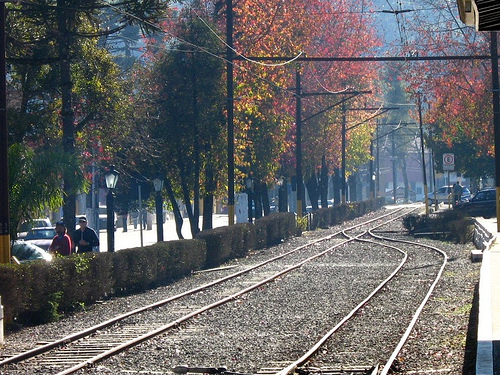
\includegraphics[width=0.33\textwidth, height=0.12\textheight]{track.jpg} & montanha, trem, inverno, frio, people, male, plant life, tree, structures, transport, car & taxi, passenger, line, transportation, railway station, passengers, railways, signals, rail, rails \\
 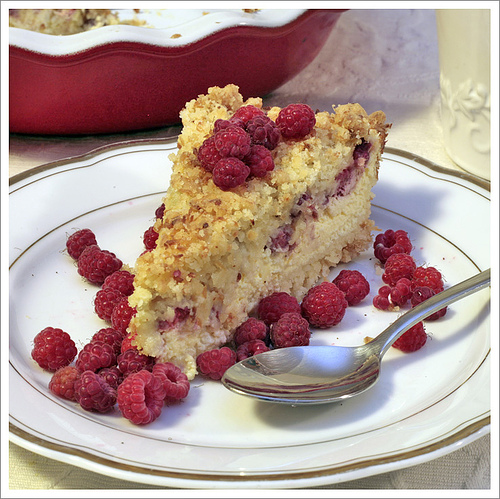
\includegraphics[width=0.33\textwidth, height=0.12\textheight]{cake.jpg} & food, raspberry, delicious, homemade & chicken, fattening, cooked, peanut, cream, cookie, house made, bread, biscuit, bakes \\

 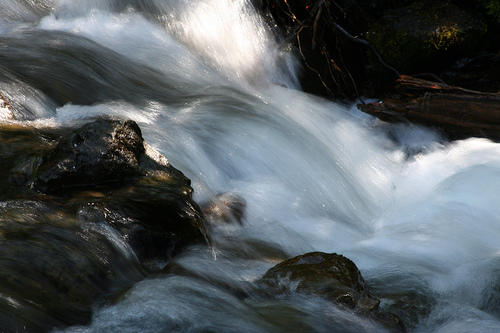
\includegraphics[width=0.33\textwidth, height=0.12\textheight]{river.jpg} & water, river & creek, lake, along, near, river, rocky, treeline, valley, woods, waters \\

 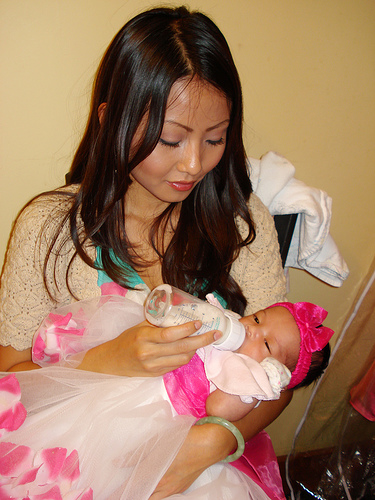
\includegraphics[width=0.33\textwidth, height=0.12\textheight]{baby.jpg} & people, portrait, female, baby, indoor & love, people, posing, girl, young, strangers, pretty, women, happy, life \\
\end{tabular}
\label{table:samples}
\caption{Samples of generated tags}
\end{table}

\section{Future Work}
本文展示的都是目前初步的结果,但是他们一方面显示了条件生成网络的潜力,另一方面这些结果本身也是很有趣并具有实用价值的应用.

我们将会在探索更多更复杂的模型,并且对这些模型的表现与特点进行更深入的分析.

%Also for many of the images, combination of their tags are more descriptive than single tags.

而且在我们目前的实验中,每一个标签都作为独立的条件变量。我们期待更进一步的研究中,如果我们把多个标签联合起来使用将会得到更好的结果。

另外一个将来可以探索的方向是为语言模型创建一个混合训练机制.类似于\cite{kiros2013multimodal}的很多工作都证实可以针对特别的任务训练有针对性的语言模型。

\subsubsection*{Acknowledgments}

这个项目是在Pylearn2~\citep{goodfellow2013pylearn2}的构架下完成的,我们对 Pylearn2的开发人员表示感谢.我们还要感谢Ian Goodfellow 在University of Montreal时与我们进行的讨论。我们还要感谢来自于Flickr的同学们的帮助(按字母排序:Andrew Stadlen, Arel Cordero, Clayton Mellina,
Cyprien Noel, Frank Liu, Gerry Pesavento, Huy Nguyen, Jack Culpepper, John Ko, Pierre Garrigues,
Rob Hess, Stacey Svetlichnaya, Tobi Baumgartner, and Ye Lu)

\small{
\bibliography{strings,strings-shorter,ml}
\bibliographystyle{natbib}}


\end{document}
